\section{Experiments}
\label{sec:simulations}

We evaluate our approach on the running example, and on a 4D flexible joint manipulator.
We implemented the RMPC controller of Alg. \ref{alg:RMPC} in MATLAB
The set computations were done using the MPT Toolbox \cite{MPT3}, and the invariant set computations using the Matlab Invariant Set Toolbox \cite{IST}. 
The reachability computations for $\oaXset{k+j}{k}$ were performed on the linear dynamics and mapped back to $x$-space as described in Sec. \ref{sec:transforming x to z}.
The RMPC optimizations were performed by Gurobi \cite{gurobi}.

\subsection{Running example}

\begin{figure}
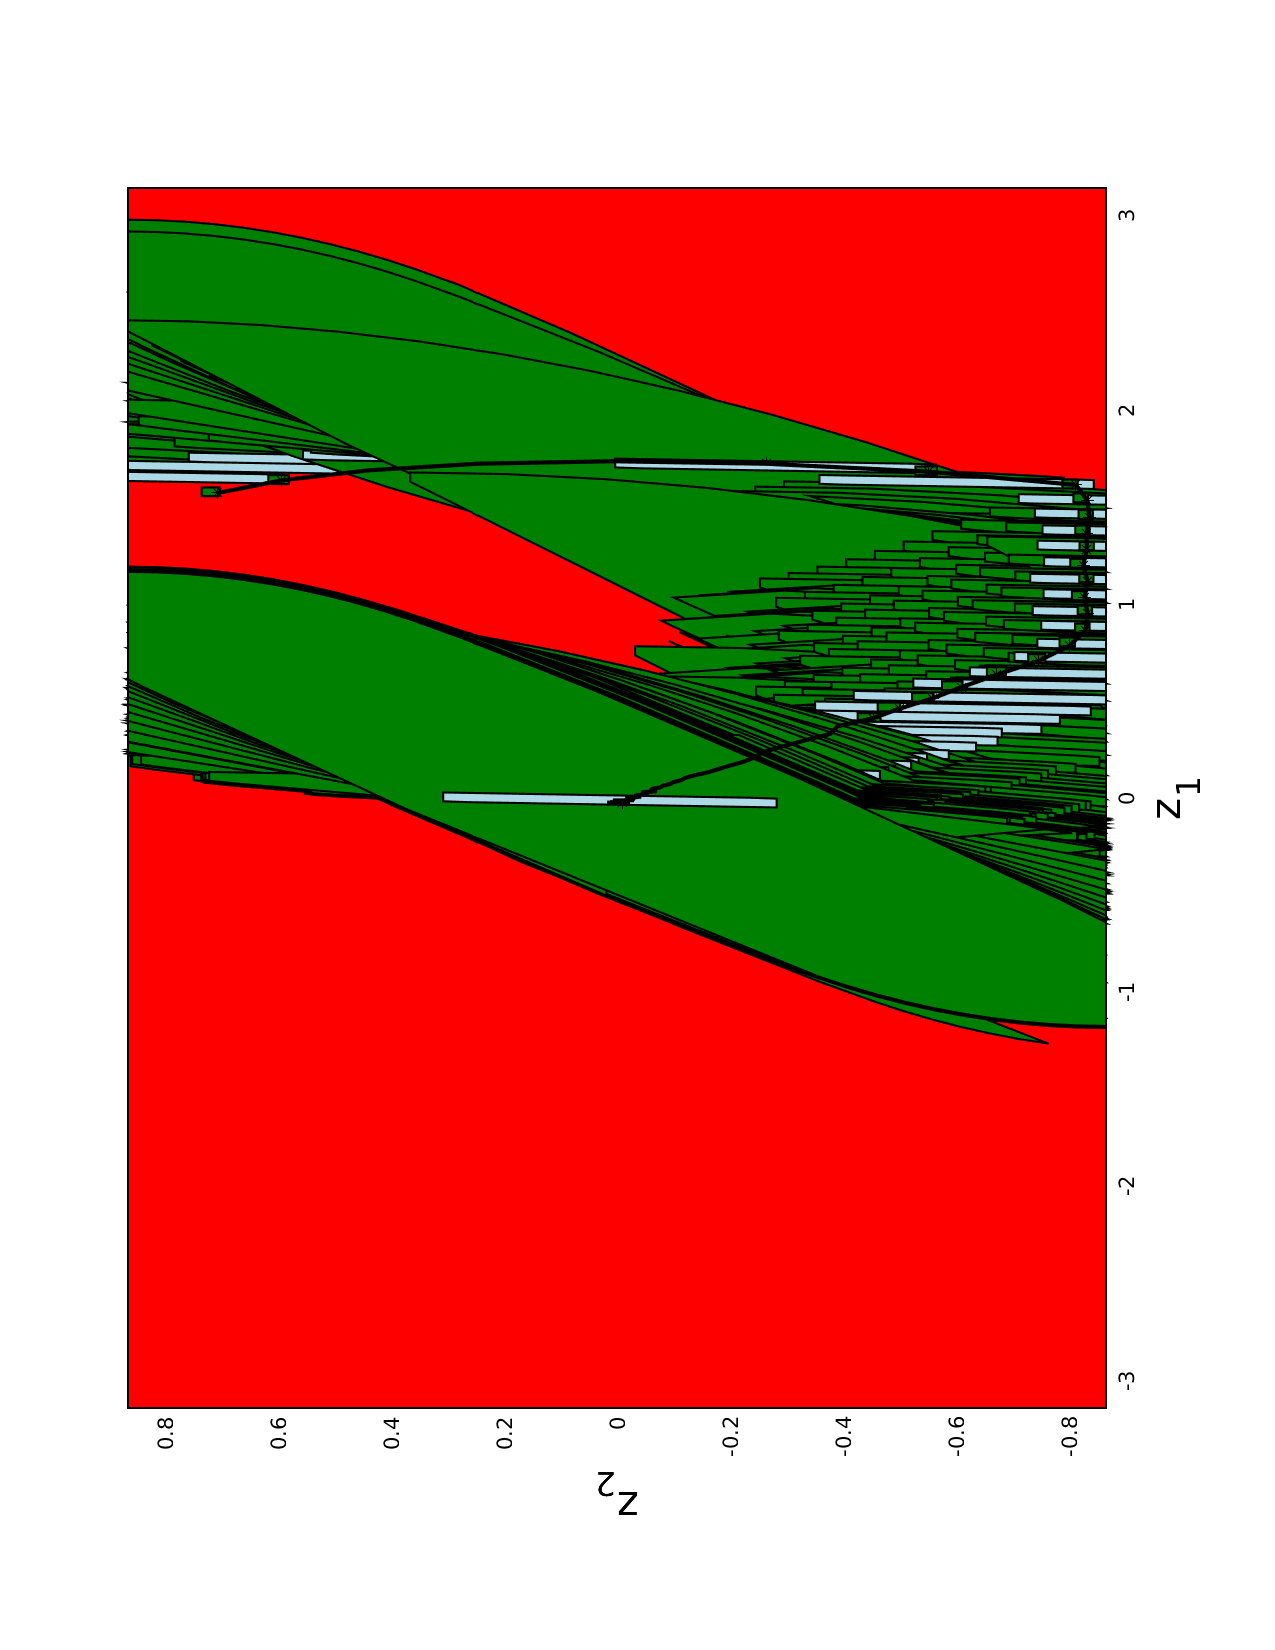
\includegraphics[angle=270,width=0.49\textwidth]{figs/z_trajectory_new_2.pdf}
\caption{Evolution of $z_1$ and $z_2$, shown by the solid black line, inside the set Z (in red). The green sets are the reach sets $\oa{Z}_{k+i|k},\forall i=1,\dotsc,N, \forall k$. The light blue set is the one step ahead reach set $\oa{Z}_{k+1|k},\forall k$.}
\label{fig:z_new_toy}
\end{figure}

\begin{figure}
	\centering	
	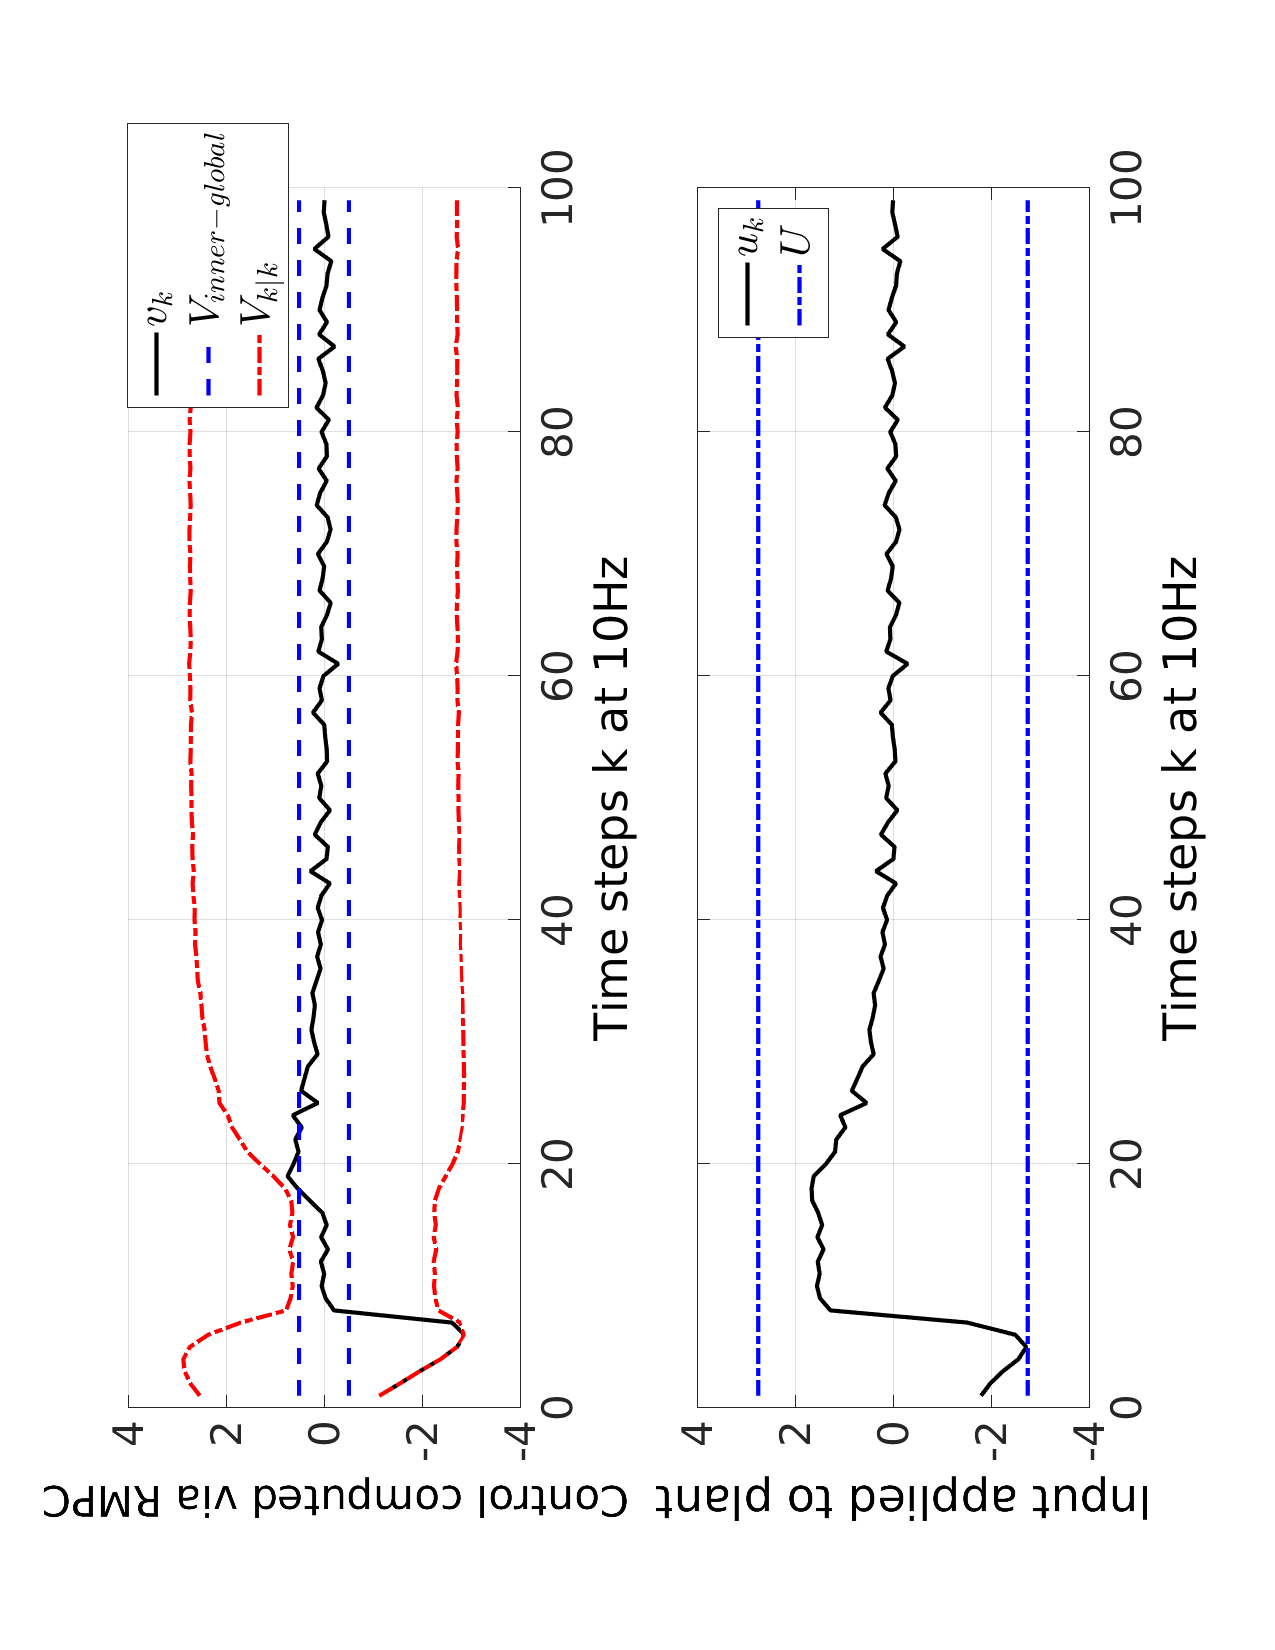
\includegraphics[width=0.49\textwidth]{figs/u_and_v_toy.pdf}
	\caption{Inputs $v$ and $u$ and their bounds for the running example.}
	\label{fig:input toy}
\end{figure}

For the running example of Eq. \ref{eq:toy_dynamics}, we discretize the feedback linearized system at 10Hz and formulate the controller with a horizon of $N=15$ steps. 
The cost function has parameters $Q=I$ and $R=10^{-2}$.
The state trajectories (and estimates) for the nonlinear and linearized systems are shown in Fig. \ref{fig:AllStates_toy}.
Note that the states converges to the equilibrium 0 (and for the running example, $T$ preserves zero). 

\begin{figure}
	\centering	
	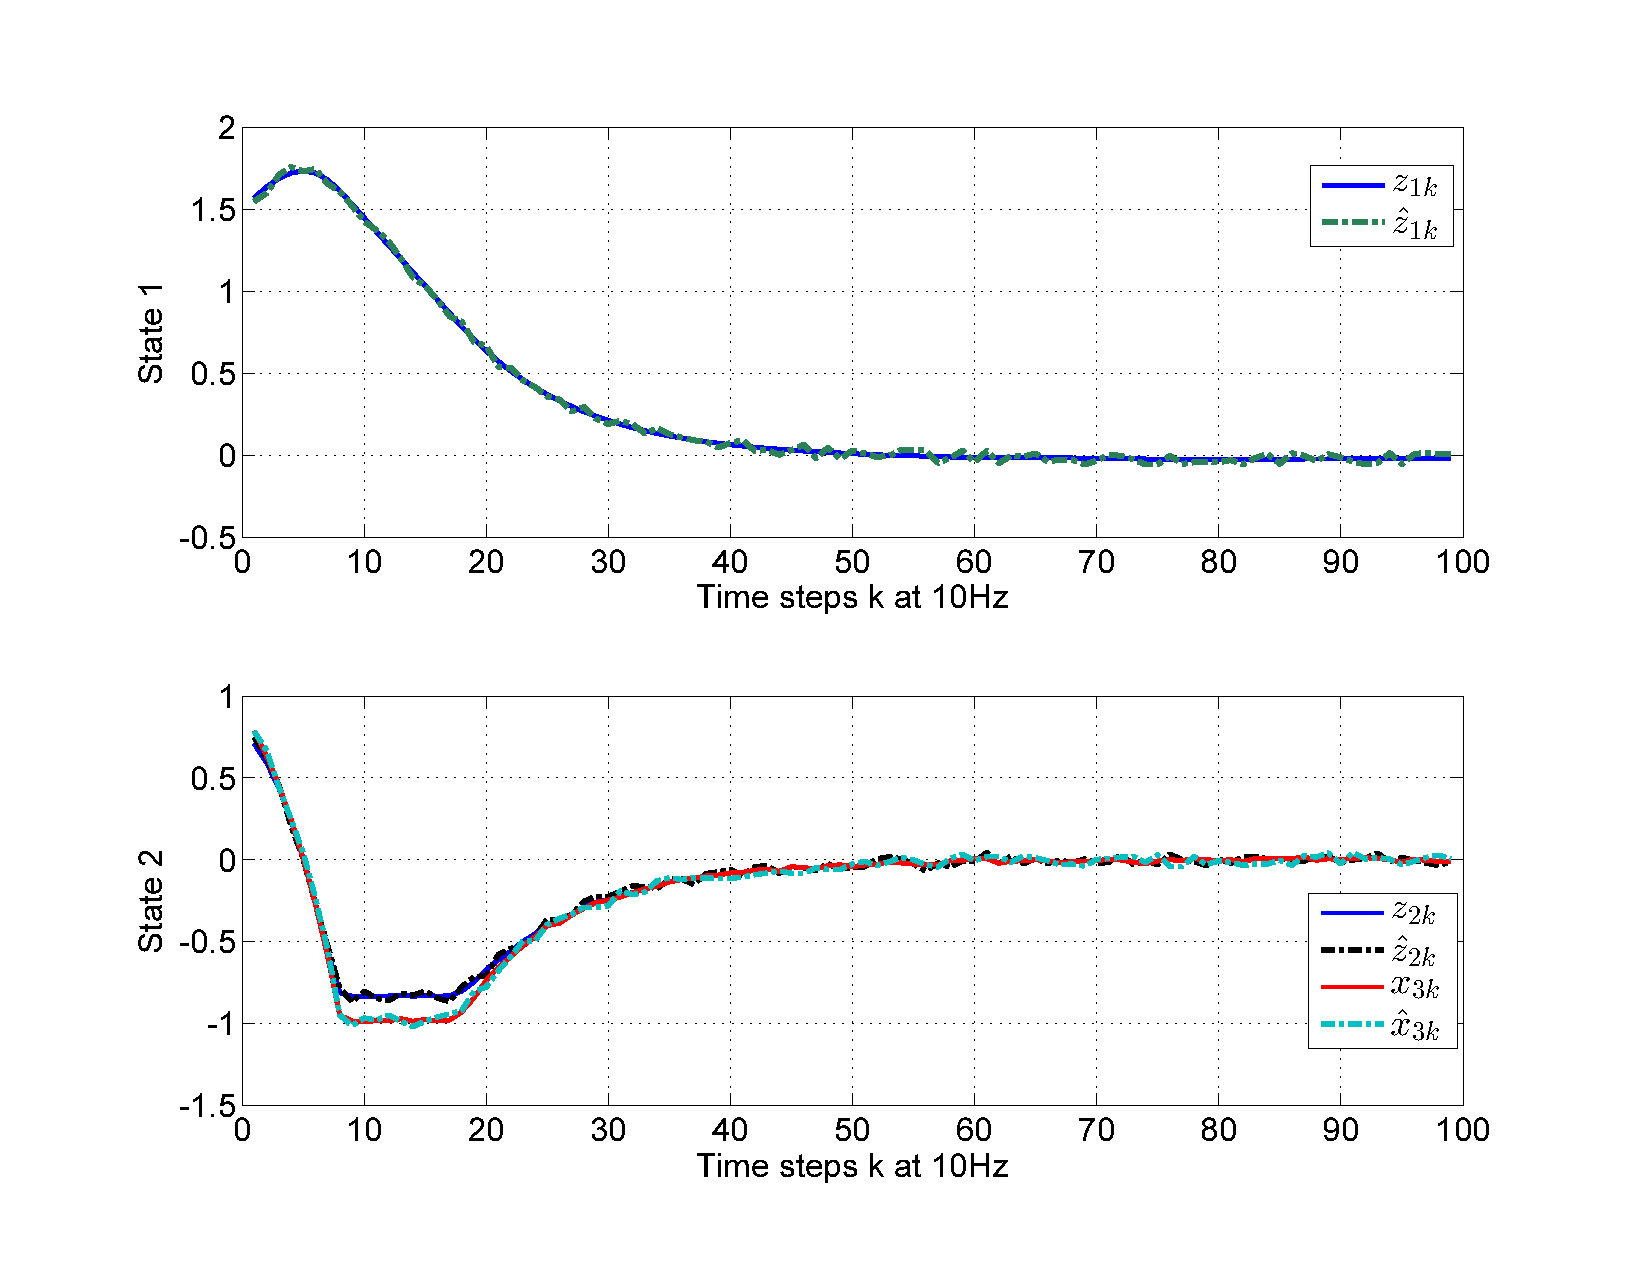
\includegraphics[width=0.49\textwidth]{figs/AllStates_toy.pdf}
	\caption{The states and their estimates of the feedback linearized and non-linear running example. Recall that $z_1 = x_1$ therefore to reduce clutter, we only plot the first state only for the feedback linearized system.}
	\label{fig:AllStates_toy}
\end{figure}




%The input for the feedback linearized system is shown in Fig. ?? along with its upper and lower rectangular bounds computed online, denoted as $\oa{V}_{k|k}$ and $\ua{V}_{k|k}$ respectively, which make up the input constraint set at time $k$.
%Also shown is the global inner approximation $V_{inner-global}$ for the input $v$. 
%It is worth noting that the bounds computed online allow for much more control action than the conservative $V_{inner-global}$. 

The input $u$ is shown in Fig. \ref{fig:input toy}, and it can be noted that $u_k \in U$ for all $k$.

\subsection{Single link flexible joint manipulator}
\label{sec:manipulator}

\begin{figure}
	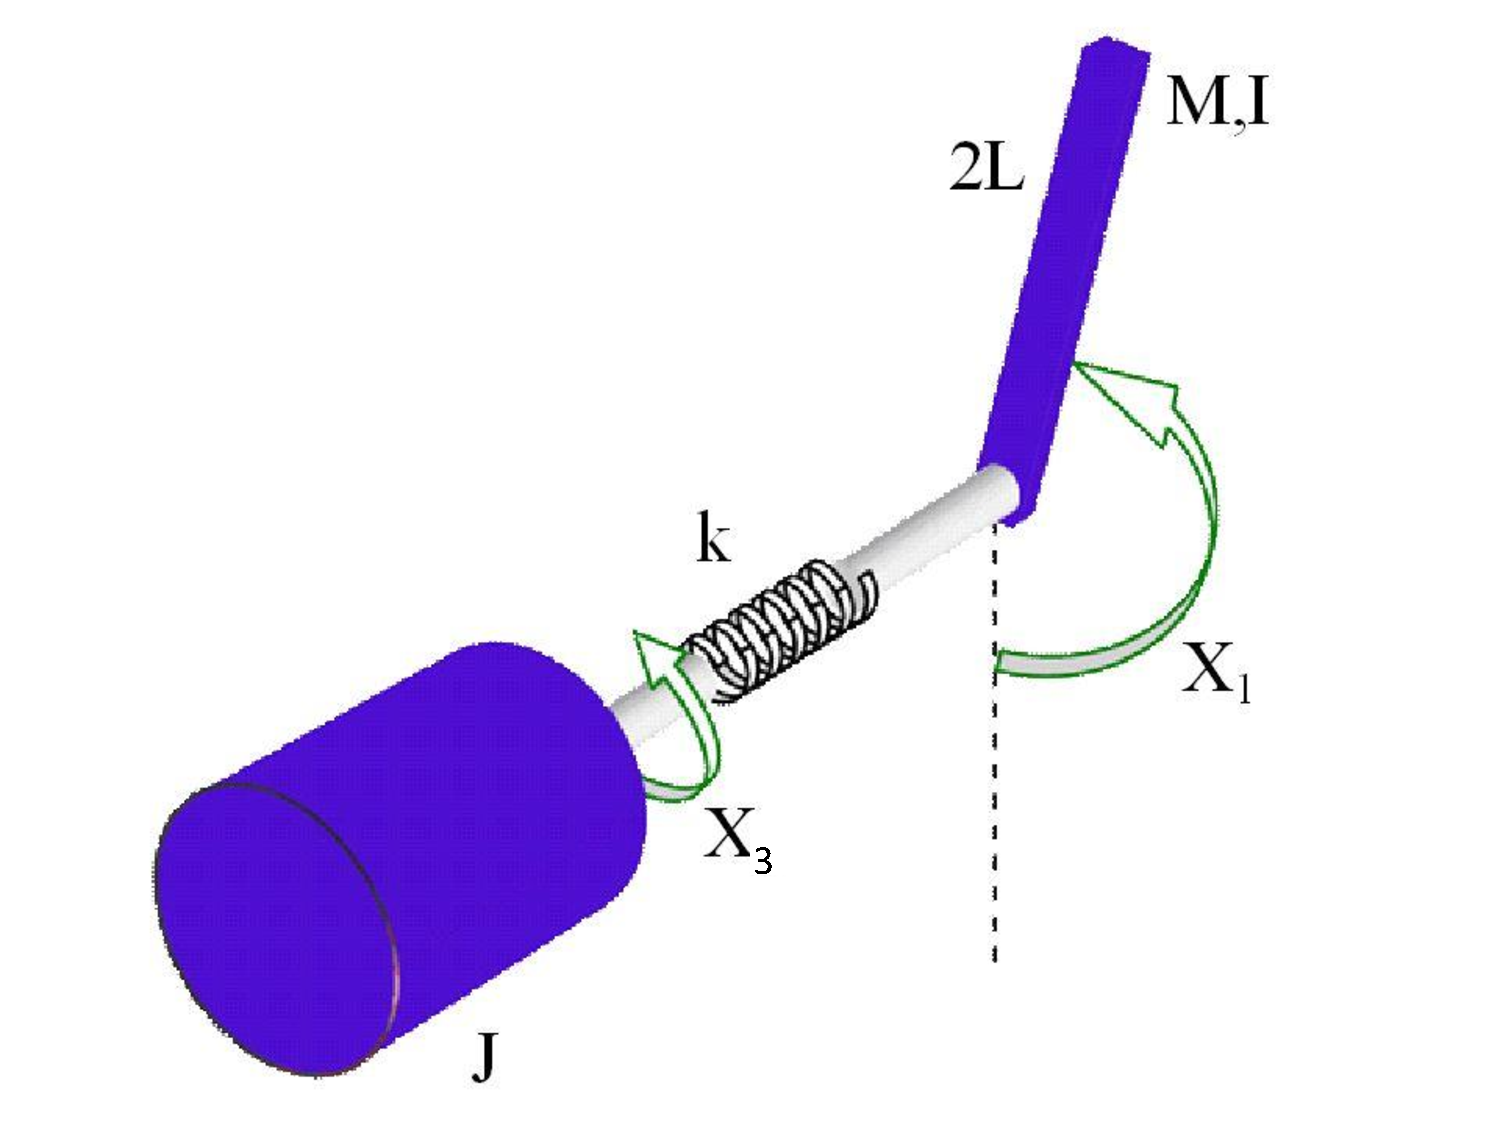
\includegraphics[scale=0.2]{figs/ManipArm.pdf}
	\caption{Flexible joint manipulator, figure from \cite{intech}.}
	\label{fig:manipulator fig}
\end{figure}

We consider the single link flexible manipulator system $S$, also used in \cite{intech}  shown in Fig. \ref{fig:manipulator fig}, whose dynamics are given by:
\begin{equation}
S: \begin{bmatrix} \dot{x}_1 \\ \dot{x}_2 \\ \dot{x}_3 \\ \dot{x}_4    \end{bmatrix} = \begin{bmatrix} x_2 \\ -\frac{mgl}{I}sin(x_1) - \frac{k}{I}(x_1-x_3)  \\ x_4 \\ \frac{k}{J}(x_1-x_3)  \end{bmatrix} + \begin{bmatrix} 0 \\ 0 \\ 0 \\ \frac{1}{J} \end{bmatrix}u
\end{equation}

This models a system where a motor, with an angular moment of inertia $J$,  is coupled to a uniform thin bar of mass $m=1/g$, length $l=1m$ and moment of inertia $I=1$, through a flexible torsional string with stiffness $k=1$. 
States $x_1$ and $x_2$ are the angles of the bar and motor shaft in radians, respectively, and $x_3, x_4$ are their respective rotational speeds in radians/sec.
The safe set is the box $X = [-\pi/4,\pi/4] \times [-\pi/4,\pi/4] \times [-\pi,\pi] \times [-\pi,\pi]$.
The input torque $u$ is bounded in $U = [\underline{u}, \overline{u}] = [-10 , 10 ]N\cdot m$. 
The estimation error $e = \hat{x} - x$ is bounded in $E = [-\pi /180, \pi /180]^4$.

The diffeomorphism $T$ is given by:
\begin{equation}
z = T(x) = \begin{bmatrix} x_1 \\ x_2 \\ -\frac{mgl}{I}sin(x_1) -\frac{k}{I}(x_1-x_3) \\ \frac{mgl}{I}x_2cos(x_1) - \frac{k}{I}(x_2-x_4)   \end{bmatrix}
\end{equation}

%For the linearization of Eq. ??, where $\hat{z}_k = z_k + M(x_k)e_k$, the matrix $M(x_k)$ is given by:
%\begin{equation}
%M(x_k) = \begin{bmatrix} 1&0&0&0 \\ 0&1&0&0 \\ -\frac{mgl}{I} cos(x_{1k}) -\frac{k}{I} &0 &\frac{k}{I} &0 \\ \frac{mgl}{I}x_{2k}sin(x_{1k}) & -\frac{mgl}{I} cos(x_{1k}) - \frac{k}{I} & 0 & \frac{k}{I}     \end{bmatrix}
%\end{equation}
The input to the feedback linearized system is given by $v=\beta u+ \alpha(x)$ where $\beta=\frac{k}{IJ} $ and 
\begin{subequations}
\label{eq:fblin_inp}
\begin{align}
\alpha(x)&=\frac{mgl}{I}x_2^2sin(x_1) + \frac{k^2}{IJ}(x_1-x_3) \nonumber \\
&- (\frac{mgl}{I}cos(x_1)-\frac{k}{I})(\frac{mgl}{I}sin(x_1)+\frac{k}{I}(x_1-x_3))
\end{align}
\end{subequations}

The feedback linearized system $S_{fl}$ has the dynamics:
$\dot{z_1} = z_2, \dot{z_2} = z_3, \dot{z_3} = z_4, \dot{z_4} = v$.
%\begin{subequations}
%\begin{align}
%\label{eq:fblin_manip}
%\dot{z_1} &= z_2 \\
%\dot{z_2} &= z_3 \\
%\dot{z_3} &= z_4 \\
%\dot{z_4} &= v
%\end{align}
%\end{subequations}


%\begin{figure}
%	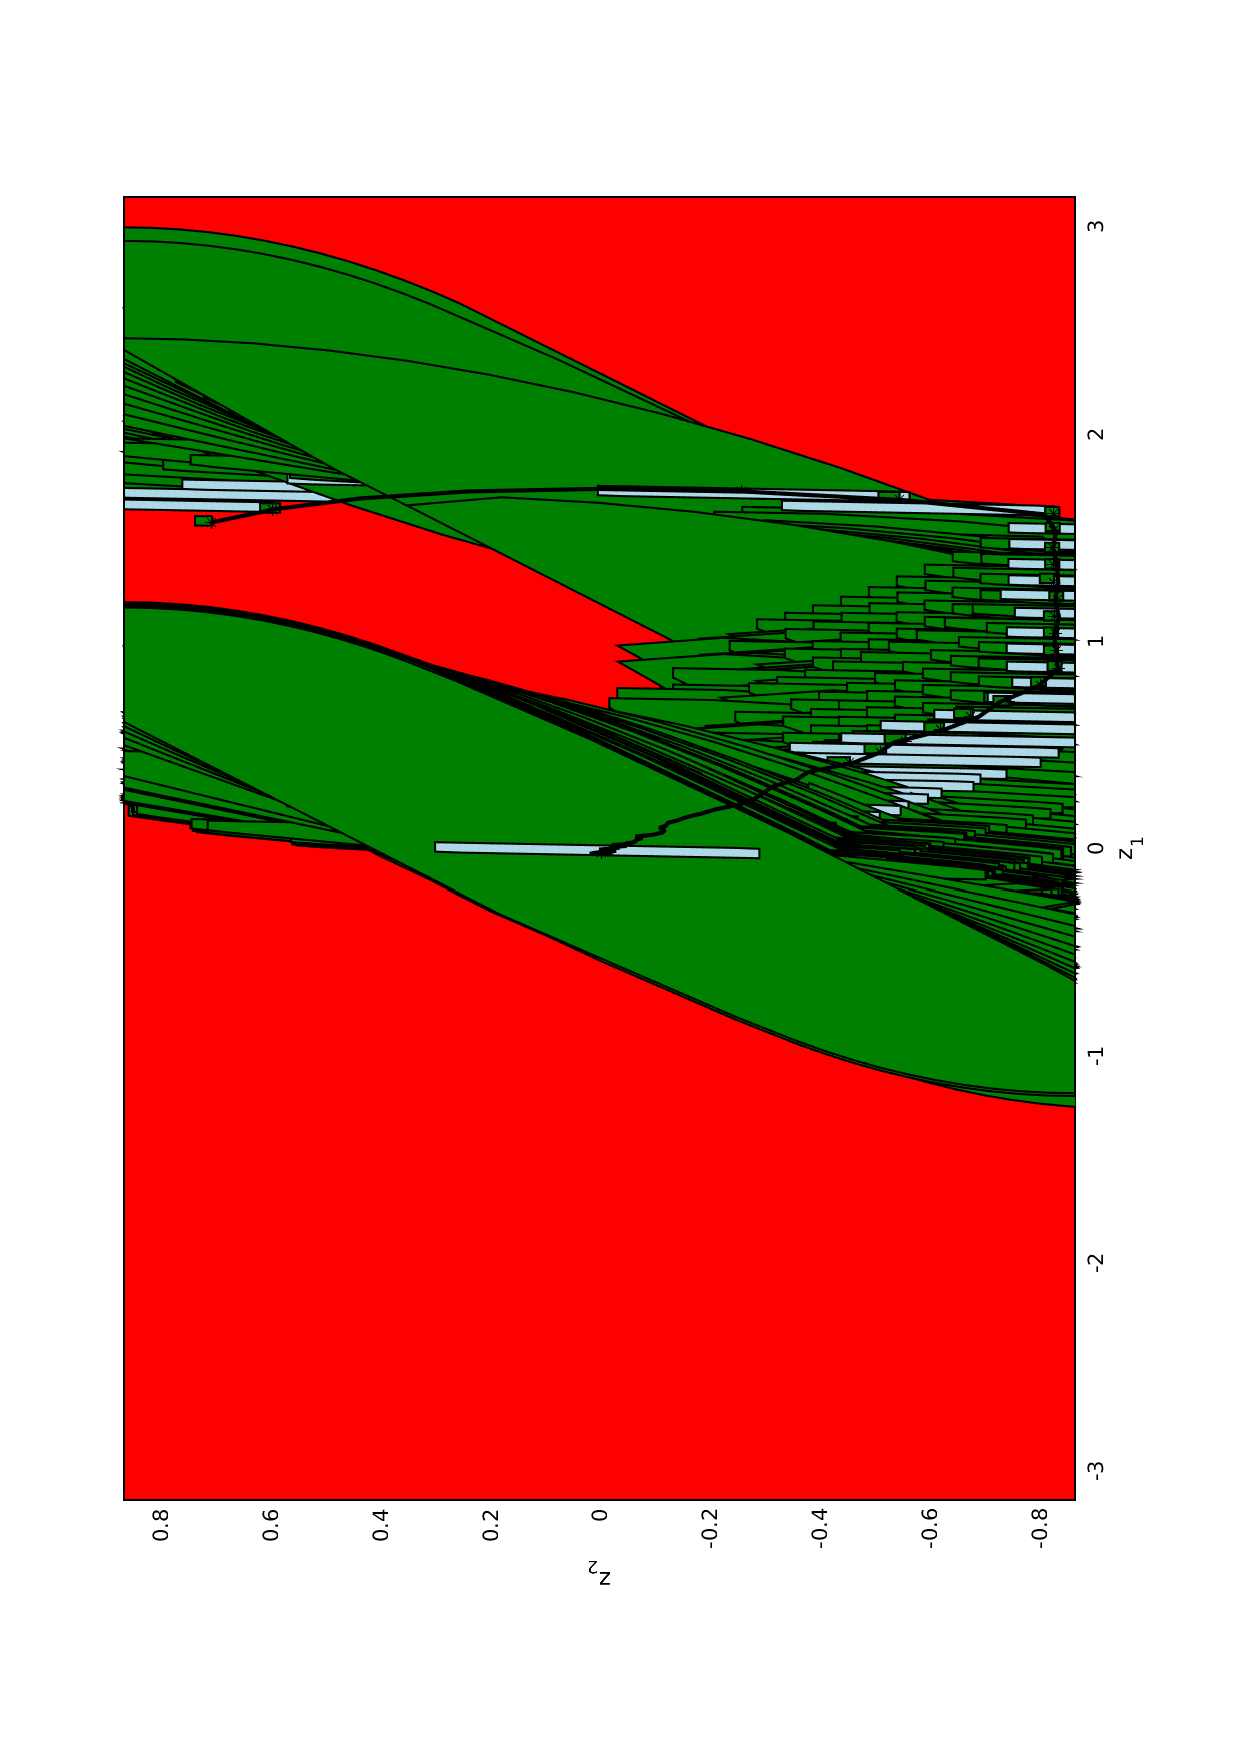
\includegraphics[angle=270,width=0.49\textwidth]{figs/z_trajectory_new.pdf}
%	\caption{Evolution of $z_1$ and $z_2$, shown by the solid black line, inside the set Z (in red). The green sets are the reach sets $\oa{Z}_{k+i|k},\forall i=1,\dotsc,N, \forall k$. The light blue set is the one step ahead reach set $\oa{Z}_{k+1|k},\forall k$.}
%	\label{fig:z_new_toy}
%\end{figure}

A global inner approximation of the $v$ input set is computed, via interval arithmetic, as $V_{inner-global} = [max_{x\in X}\alpha(x) + \beta \underline{u}, min_{x\in X}\alpha(x) + \beta \overline{u}]$. 
Similarly, the inner approximations $\ua{V}_{k+j|k}$ are computed online by interval arithmetic as $\ua{V}_{k+j|k} = [max_{x\in \oa{X}_{k+j|k}} \alpha(x) + \beta \underline{u},  min_{x\in \oa{X}_{k+j|k}}\alpha(x) + \beta \overline{u}]$. 
Using the procedure of Sec. \ref{sec:transforming x to z} the set of states for $S_{fl}$ is given by $Z = [-0.5121, 0.5121]^2 \times [-2.5347, 2.5347] \times [-2.5603, 2.5603]$.

We applied our controller to the above system with a discretization rate of 10Hz and MPC horizon $N=10$.
Fig.\ref{fig:AllStates_manip} show the states of the feedback linearized system $S_{fl}$. 
They converge to the origin in the presence of estimation error, while respecting all constraints.
Fig. \ref{fig:AllStates_manip} also shows $x_3$ and $x_4$: they also converge to zero (and remember $x_1 = z_1$ and $x_2 = z_2$).

\begin{figure}
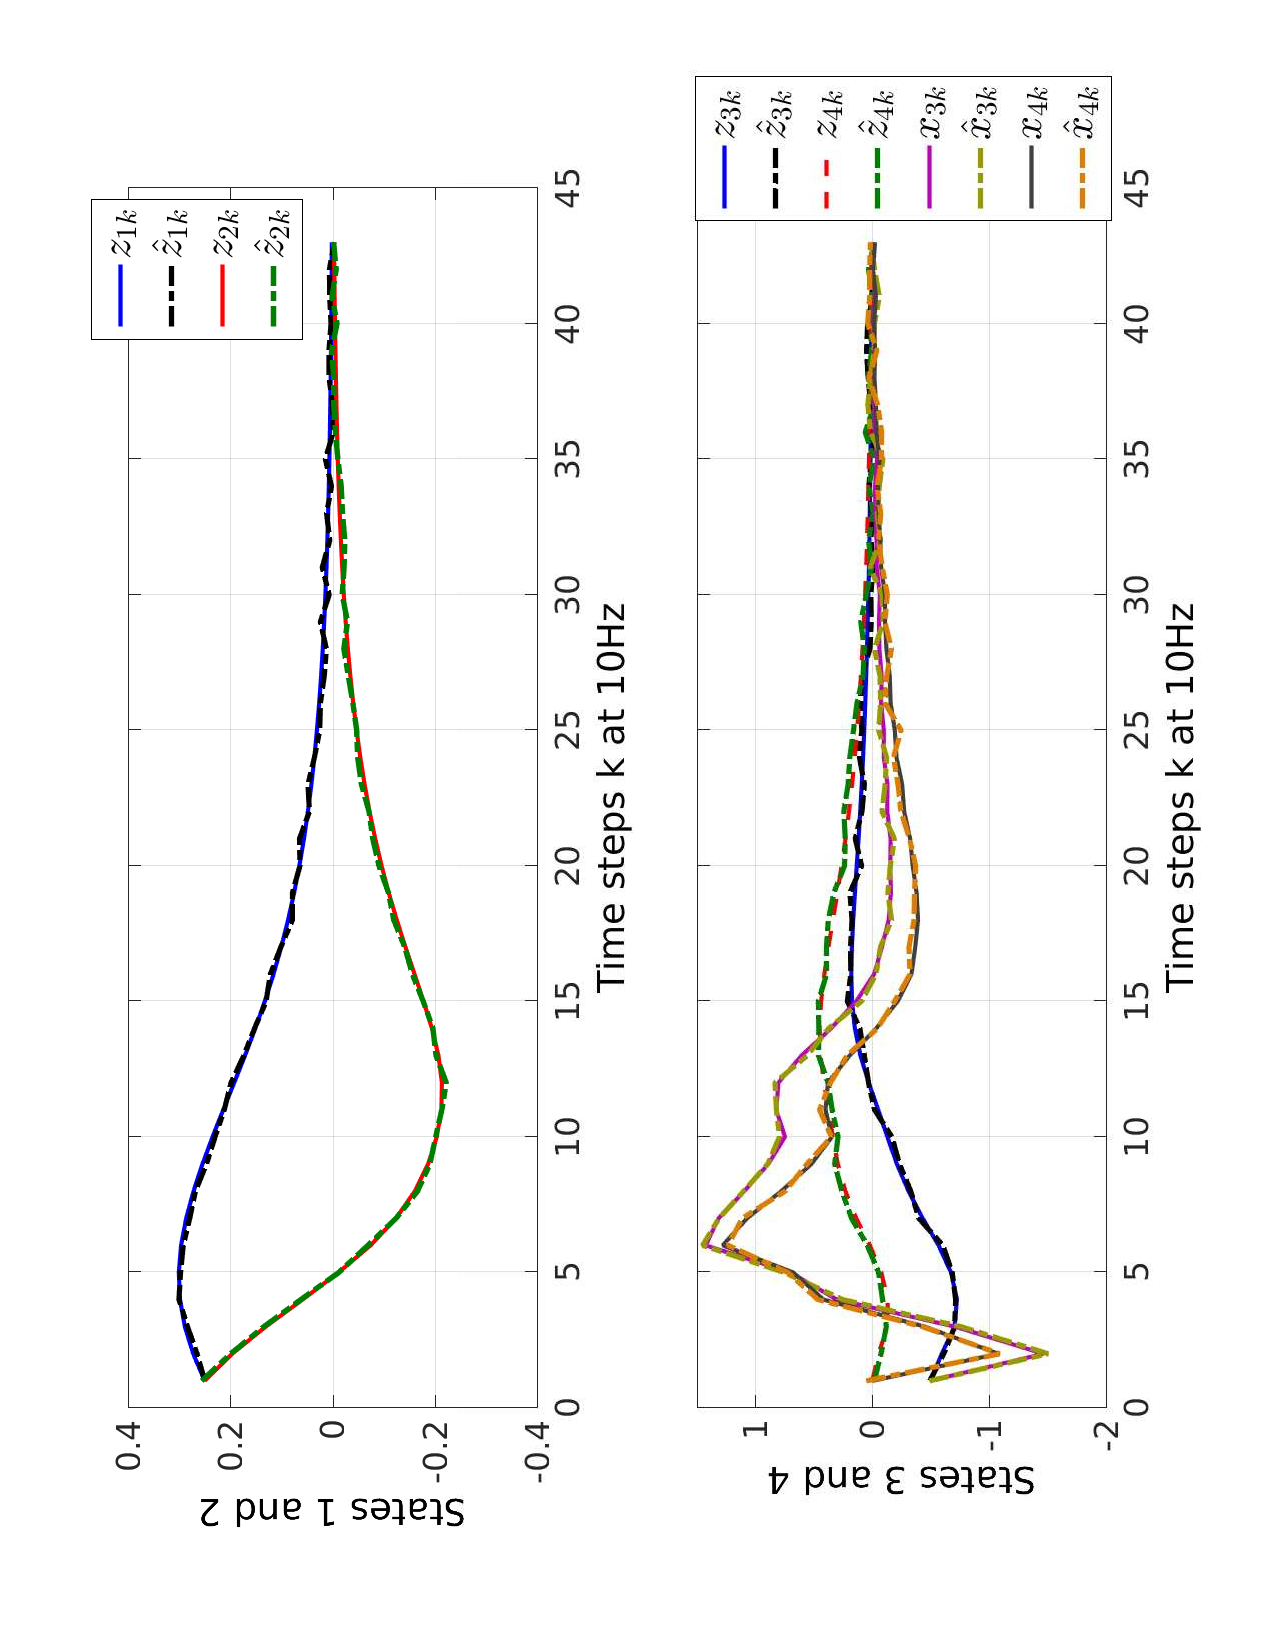
\includegraphics[width=0.49\textwidth]{figs/AllStates_manip.pdf}
\caption{The states and their estimates of the feedback linearized and non-linear manipulator. Recall that $z_1 = x_1$ and $z_2=x_2$, therefore to reduce clutter, we only plot first two states only for the feedback linearized system.}
\label{fig:AllStates_manip}
\end{figure}

%\begin{figure}
%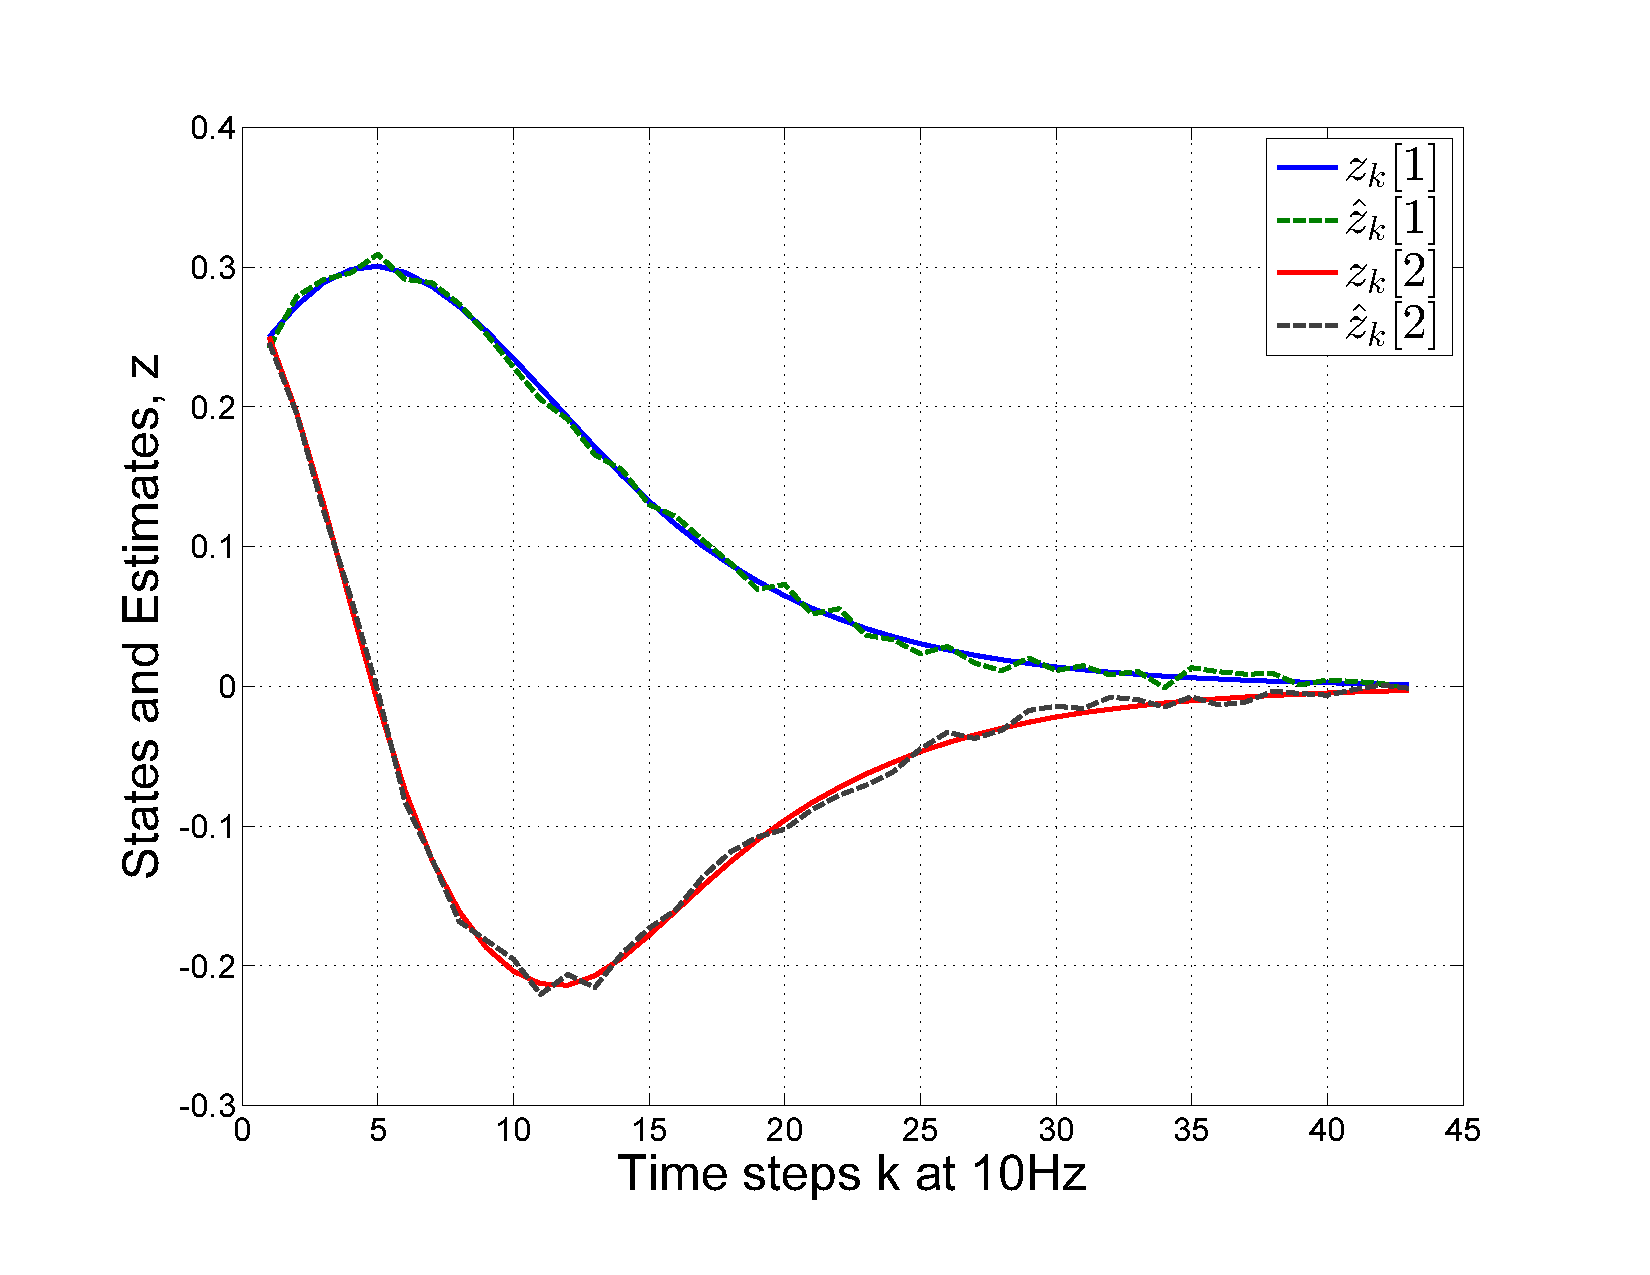
\includegraphics[width=0.49\textwidth]{figs/z_1n2_manip.pdf}
%\caption{$z_1$ and $z_2$ and their estimates $\hat{z_1}, \, \hat{z_2}$ vs time. Recall $z_1=x_1, z_2 = x_2$.}
%\label{fig:z_12}
%\end{figure}


%\begin{figure}
%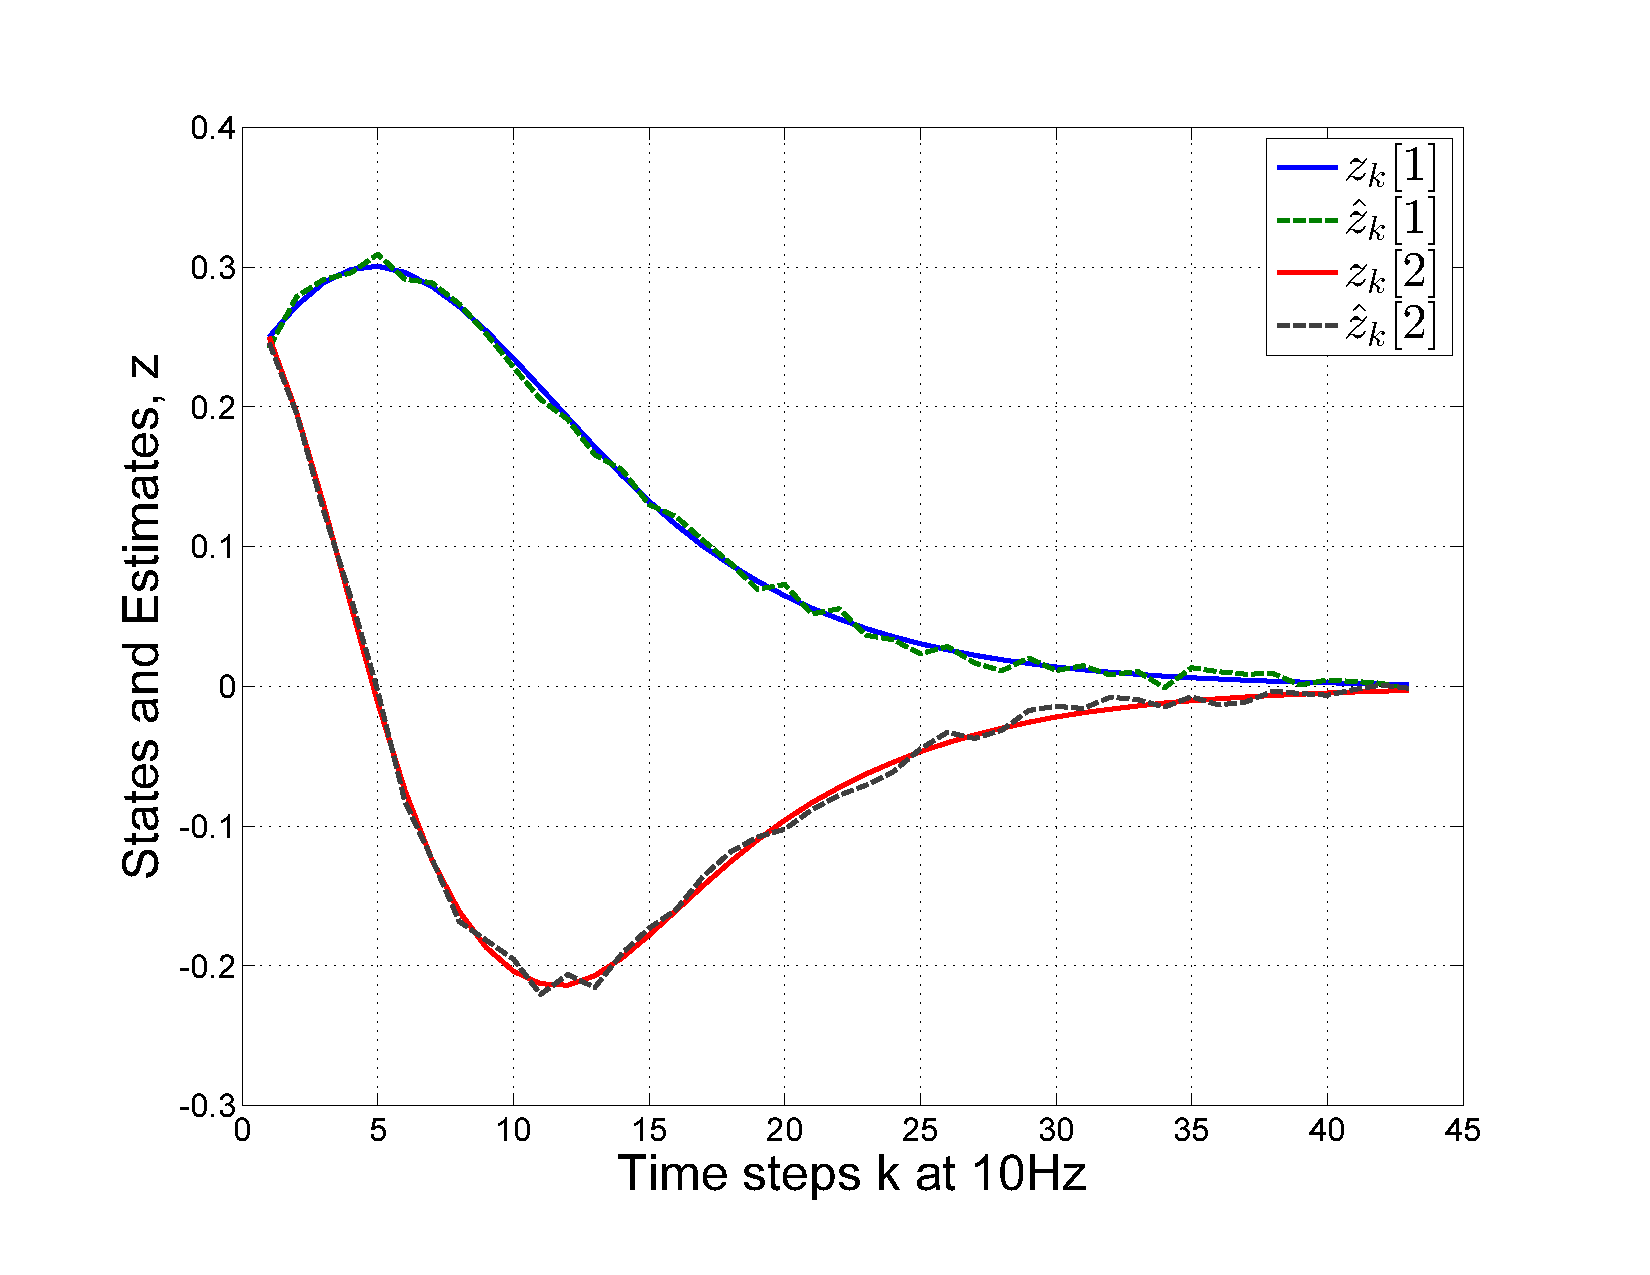
\includegraphics[width=0.49\textwidth]{figs/z_1n2_manip.pdf}
%\caption{$z_1$ and $z_2$ and their estimates $\hat{z_1}, \, \hat{z_2}$ vs time. Recall $z_1=x_1, z_2 = x_2$.}
%\label{fig:z_12}
%\end{figure}

%\begin{figure}
%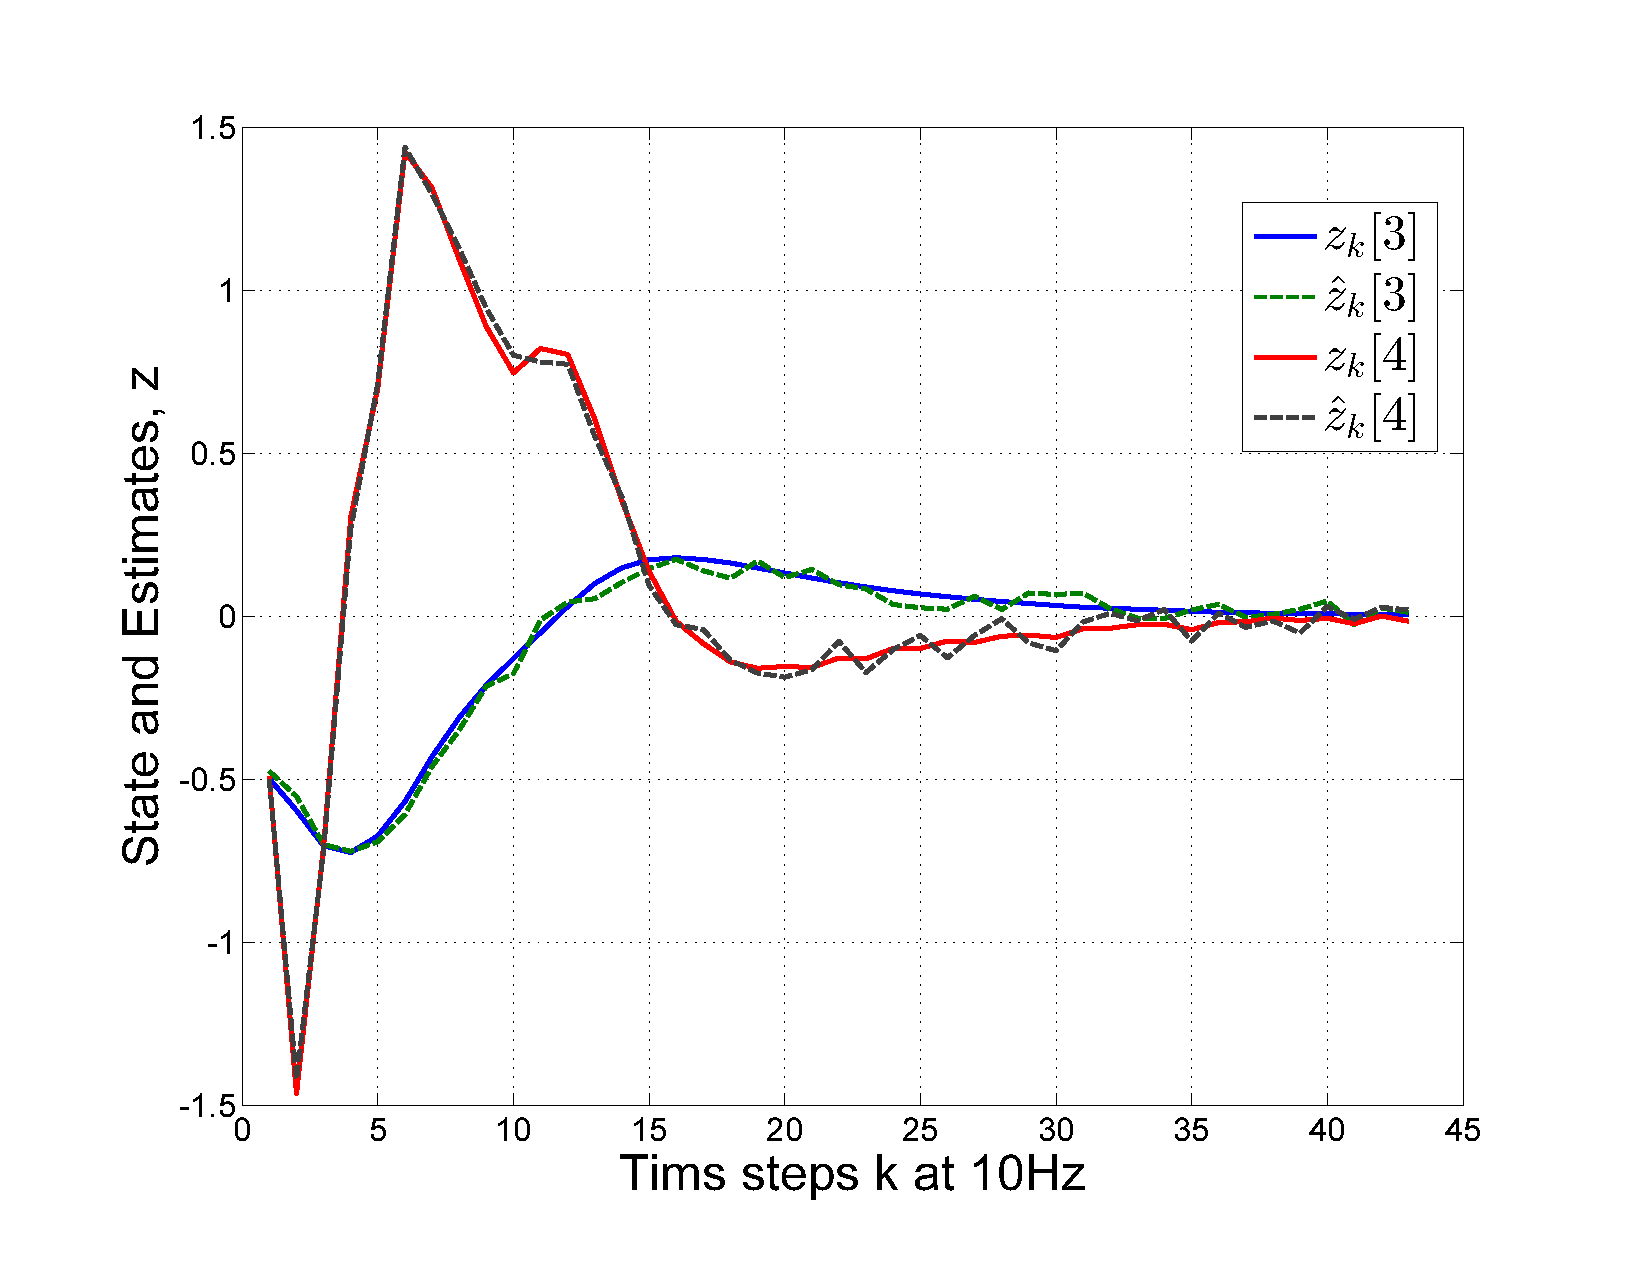
\includegraphics[width=0.49\textwidth]{figs/z_3n4_manip.pdf}
%\caption{$z_3$ and $z_4$ and their estimates $\hat{z_3}, \, \hat{z_4}$ vs time. }
%\label{fig:z_34}
%\end{figure}

Fig. \ref{fig:v_and_limits} shows the input $v$ to $S_{fl}$ $v$ along with the global inner approximation $V_{inner-global}$ and the $x$-dependent inner approximations $\ua{V}_{k+k|k}$ computed online.
Note that the bounds computed online allow for significantly more control action compared to the conservative global inner approximation. 
Finally, Fig. \ref{fig:v_and_limits} also shows the input $u$ applied to the non-linear system (and its bounds), which robustly respects its constraints $u \in U$.

%\begin{figure}
%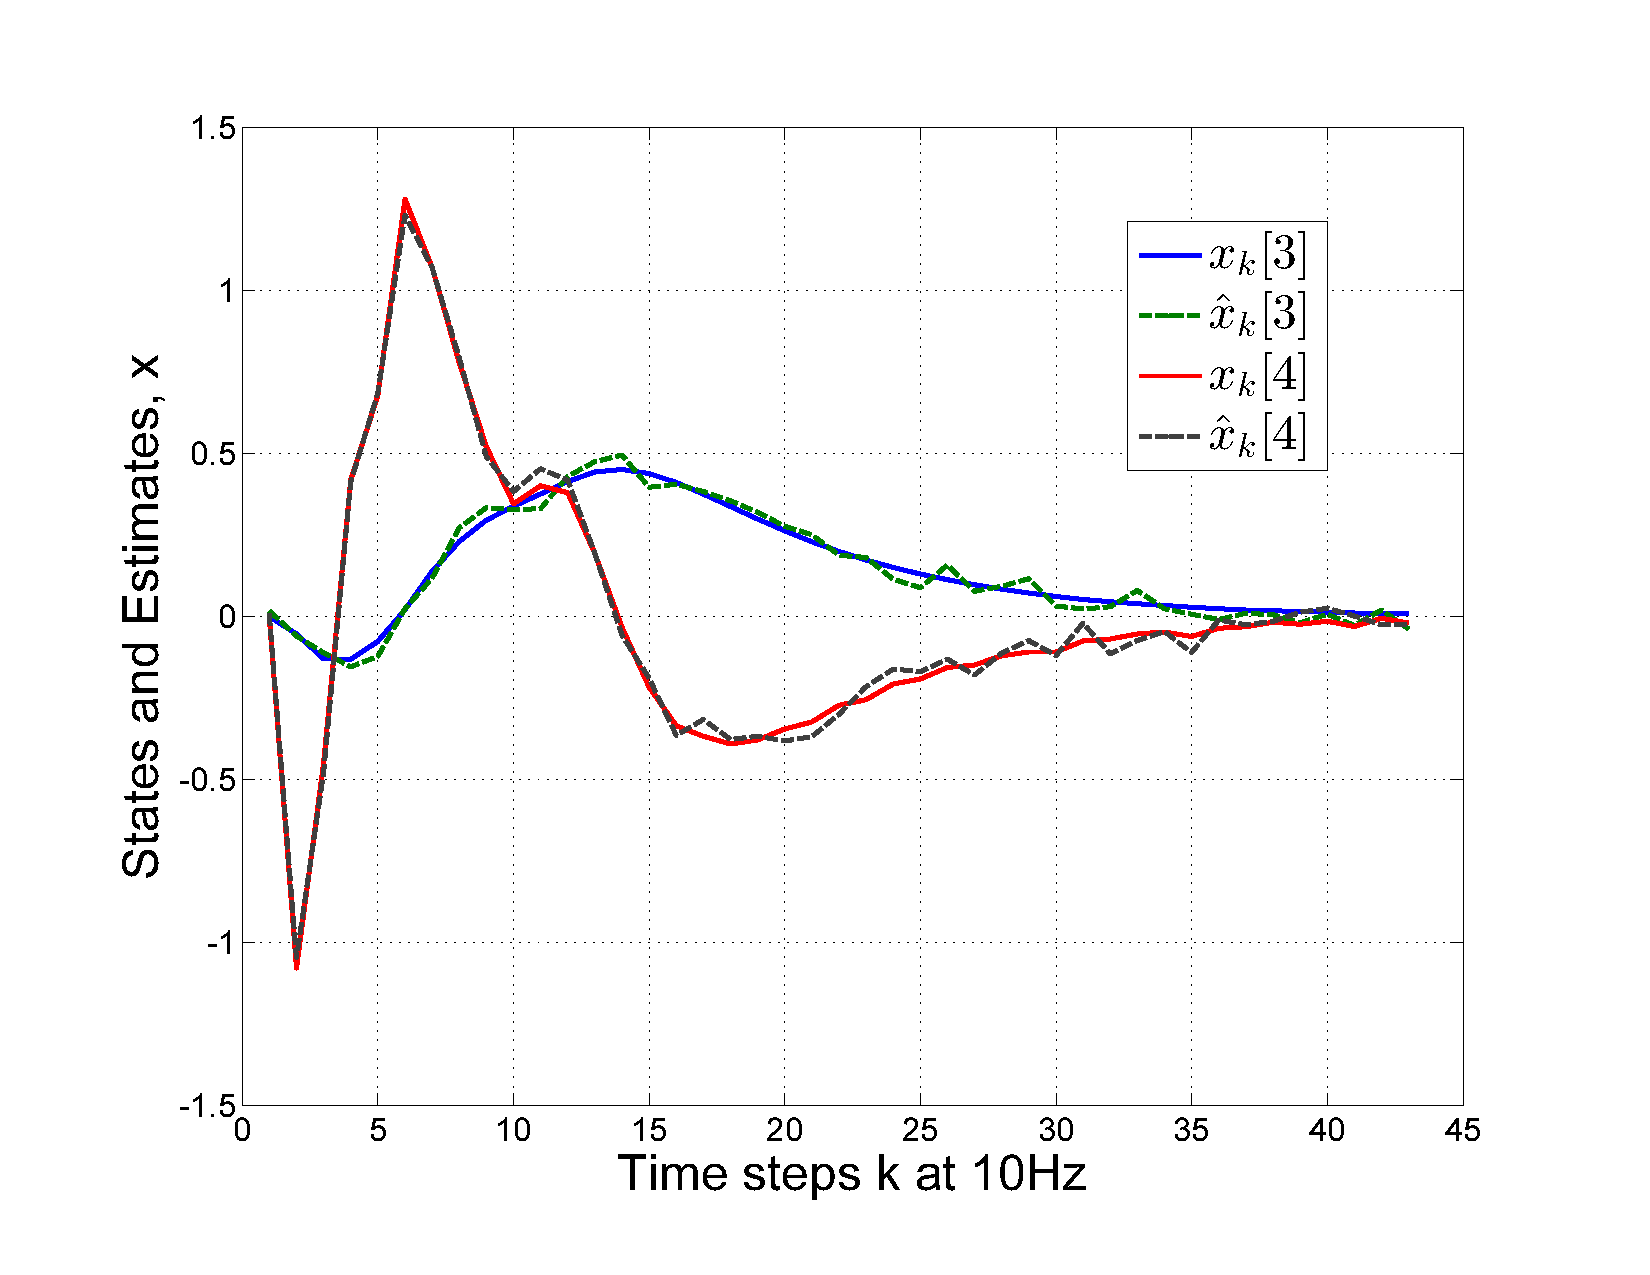
\includegraphics[width=0.49\textwidth]{figs/x_3n4_manip.pdf}
%\caption{$x_3$ and $x_4$ and their estimates $\hat{x_3}, \, \hat{x_4}$ vs time. }
%\label{fig:x_34}
%\end{figure}


\begin{figure}
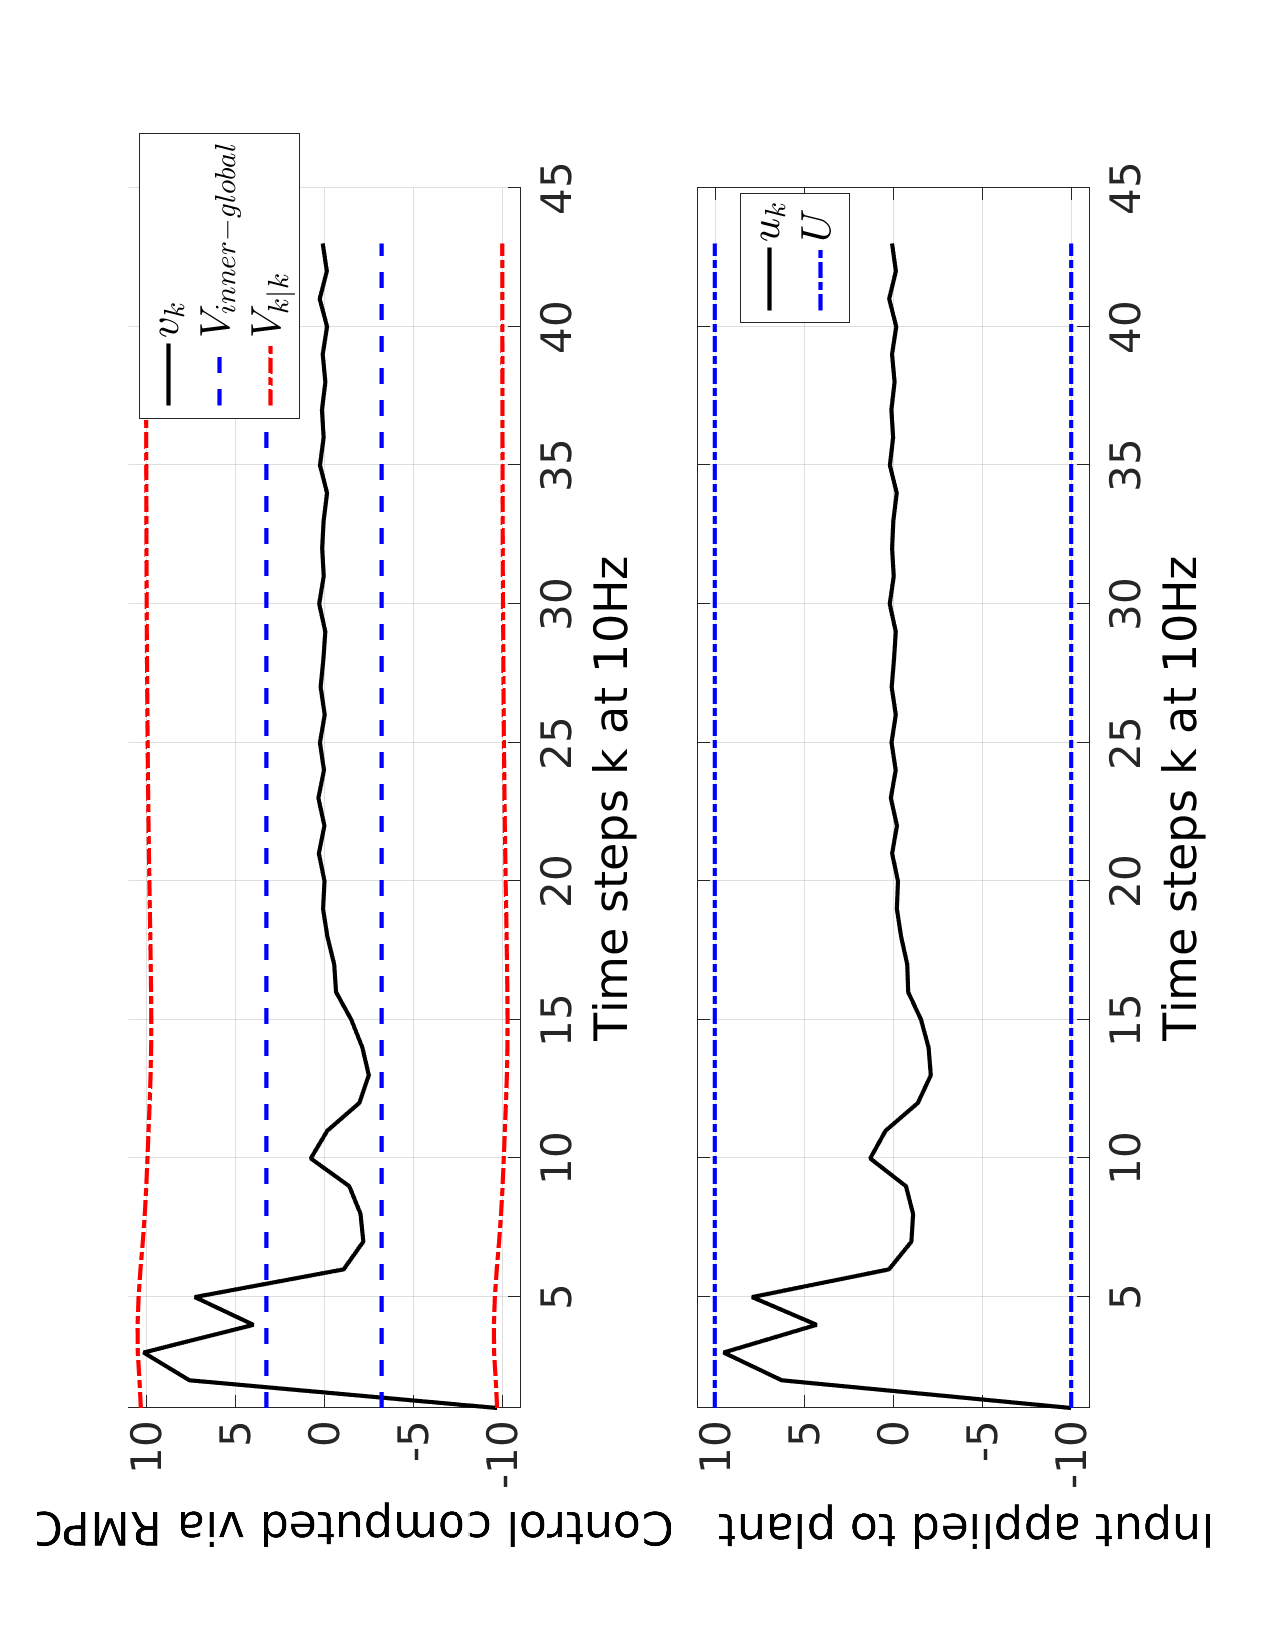
\includegraphics[width=0.49\textwidth]{figs/u_and_v_manip.pdf}
\caption{Inputs $v$ and $u$ and their bounds for the manipulator example .}
\label{fig:v_and_limits}
\end{figure}



%\begin{figure}
%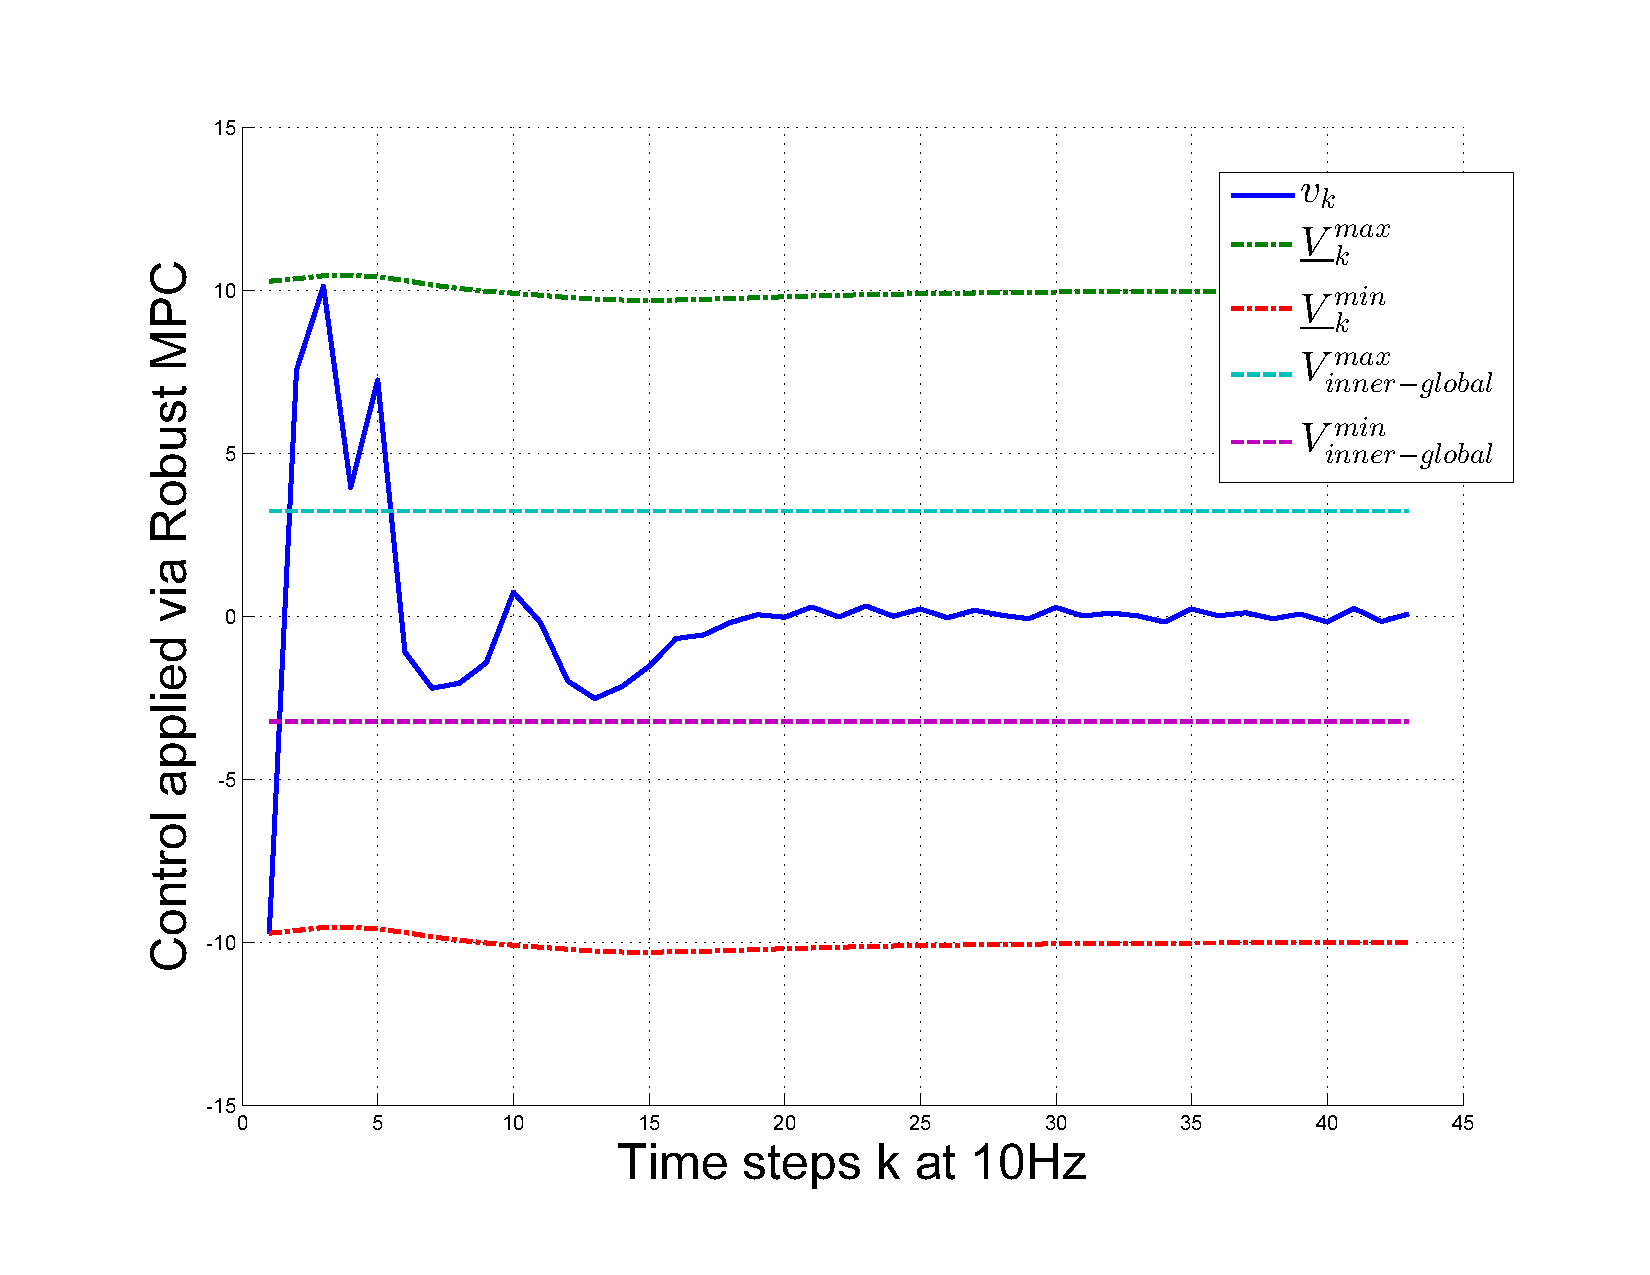
\includegraphics[width=0.49\textwidth]{figs/v_and_limits_manip.pdf}
%\caption{Input to the feedback linearized system and its bounds.}
%\label{fig:v_and_limits}
%\end{figure}

%\begin{figure}
%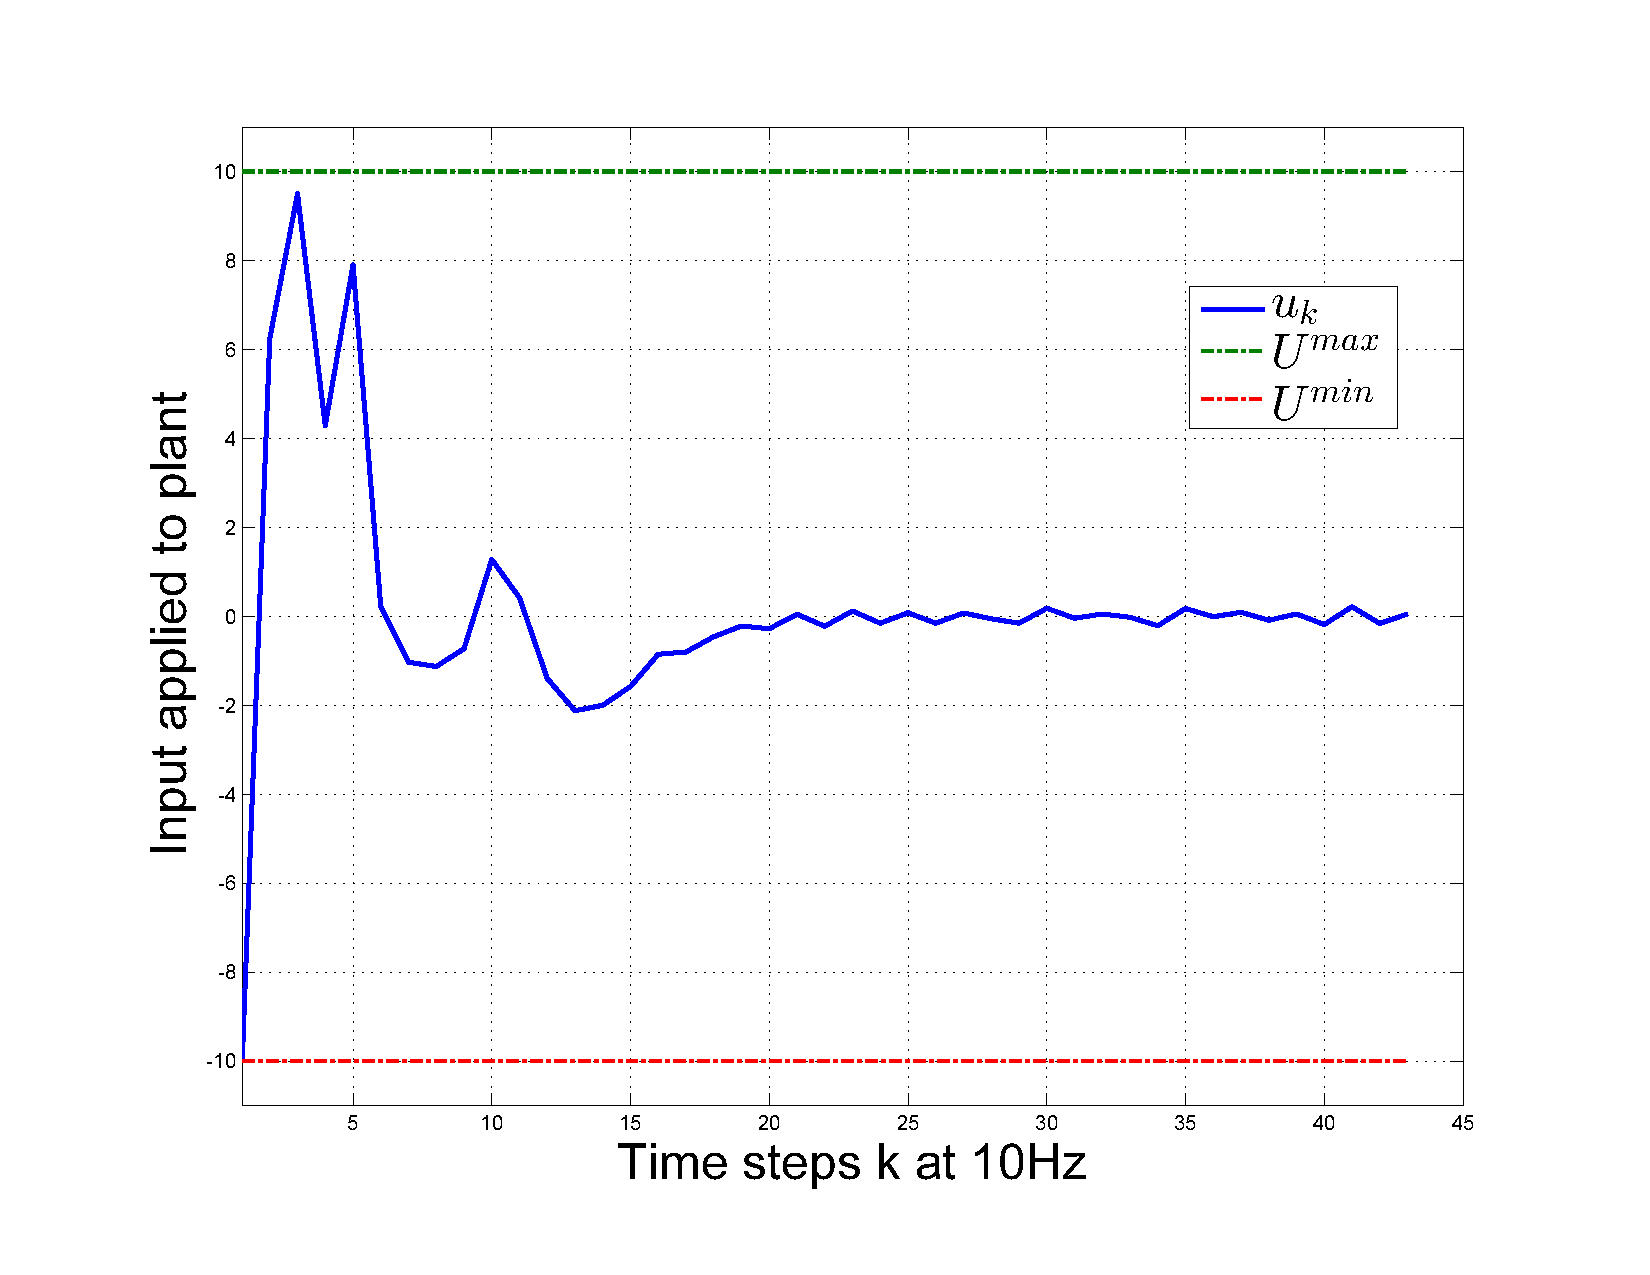
\includegraphics[width=0.49\textwidth]{figs/u_and_limits_manip.pdf}
%\caption{Input to the non-linear system and its upper and lower limits.}
%\label{fig:u_and_limits}
%\end{figure}


